\documentclass[a4paper,11pt]{article}
% ============================================================
%  preamble_documents.tex
%  article / report / book 클래스 공용 프리앰블 (XeLaTeX 기준)
%  수식·기호, TikZ, 표, 한글 지원에 필요한 패키지를 모아둔다.
% ============================================================

% ---------------------------------------------------------------
% 페이지 레이아웃
% ---------------------------------------------------------------
\usepackage[a4paper, margin=2.5cm]{geometry}
\usepackage{setspace}
\onehalfspacing
\usepackage{microtype}      % 자간/자폭 미세 조정
\usepackage{csquotes}       % 올바른 인용부호

% ---------------------------------------------------------------
% 한글 / 폰트 (XeLaTeX + kotex)
% ---------------------------------------------------------------
\usepackage{fontspec}
\usepackage{kotex}
% 한글 폰트를 직접 지정하려면 아래 주석을 해제해서 사용한다.
% \setmainhangulfont{Noto Serif CJK KR}
% \setsanshangulfont{Noto Sans CJK KR}
% \setmonohangulfont{Noto Sans Mono CJK KR}

% ---------------------------------------------------------------
% 수식 & 기호
% ---------------------------------------------------------------
\usepackage{amsmath, amssymb, amsthm}
\usepackage{mathtools}      % amsmath 확장 (\coloneqq, \DeclarePairedDelimiter 등)
\usepackage{bm}             % 굵은 수식 기호 \bm{}
\usepackage{mathrsfs}       % 필기체 글꼴 \mathscr{}
\usepackage{cancel}         % \cancel, \xcancel, \bcancel
\usepackage{esint}          % 다양한 적분 기호 (\oiint 등)
\IfFileExists{siunitx.sty}{\usepackage{siunitx}}{}  % 단위/숫자 표기 \si{}, \num{} (있을 때만)
\IfFileExists{physics.sty}{\usepackage{physics}}{}  % \dv, \pdv, \abs, \norm 등 (있을 때만)

% 자주 쓰는 수식 매크로
\DeclarePairedDelimiter{\abs}{\lvert}{\rvert}
\DeclarePairedDelimiter{\norm}{\lVert}{\rVert}
\newcommand{\R}{\mathbb{R}}
\newcommand{\N}{\mathbb{N}}
\newcommand{\Z}{\mathbb{Z}}
\newcommand{\Q}{\mathbb{Q}}
\newcommand{\C}{\mathbb{C}}

% ---------------------------------------------------------------
% 정리/정의 환경 (한글 표기)
% ---------------------------------------------------------------
\theoremstyle{plain}
\newtheorem{theorem}{정리}[section]
\newtheorem{lemma}[theorem]{보조정리}
\newtheorem{corollary}[theorem]{따름정리}
\newtheorem{proposition}[theorem]{명제}
\theoremstyle{definition}
\newtheorem{definition}[theorem]{정의}
\newtheorem{example}[theorem]{예제}
\theoremstyle{remark}
\newtheorem*{remark}{참고}

% ---------------------------------------------------------------
% 표
% ---------------------------------------------------------------
\usepackage{array}
\usepackage{booktabs}
\usepackage{multirow}
\usepackage{multicol}
\usepackage{tabularx}
\usepackage{longtable}
\usepackage{makecell}

% ---------------------------------------------------------------
% 그림 & TikZ
% ---------------------------------------------------------------
\usepackage{graphicx}
\usepackage{xcolor}
\usepackage{caption}
\usepackage{subcaption}
\usepackage{float}
\usepackage{tikz}
\usepackage{tikz-cd}
\usepackage{pgfplots}
\pgfplotsset{compat=1.18}
\usetikzlibrary{
  arrows.meta,
  calc,
  positioning,
  shapes.geometric,
  shapes.symbols,
  fit,
  backgrounds,
  patterns,
  matrix,
  intersections,
  decorations.pathmorphing,
  decorations.markings,
  angles,
  quotes
}
\tikzset{
  >=stealth,
  line cap=round,
  line join=round,
  every picture/.style={line width=0.9pt},
  box/.style={draw, rounded corners, minimum width=2.8cm, minimum height=1.2cm, align=center},
  circlebox/.style={draw, circle, minimum size=1cm, align=center},
  arrow/.style={->, thick},
  dashedarrow/.style={->, thick, dashed},
  point/.style={circle, fill, inner sep=1.2pt},
  gridhelp/.style={help lines, gray!35},
  highlight/.style={fill=blue!10, draw=blue!60!black}
}

% ---------------------------------------------------------------
% 목록 & 코드
% ---------------------------------------------------------------
\usepackage{enumitem}
\usepackage{listings}
\lstset{
  basicstyle=\ttfamily\small,
  breaklines=true,
  columns=fullflexible,
  frame=single,
  numbers=left,
  numberstyle=\tiny,
  tabsize=2,
}

% ---------------------------------------------------------------
% 하이퍼링크 & 상호참조
% ---------------------------------------------------------------
\usepackage[hidelinks]{hyperref}
\usepackage{cleveref}

% ---------------------------------------------------------------
% 머리말/꼬리말
% ---------------------------------------------------------------
\usepackage{fancyhdr}
\setlength{\headheight}{14pt}
\pagestyle{fancy}
\fancyhf{}
\fancyhead[R]{\nouppercase{\rightmark}}
\fancyfoot[C]{\thepage}
\renewcommand{\headrulewidth}{0.4pt}


\title{Article 템플릿}
\author{Master}
\date{\today}

\begin{document}

\maketitle

\begin{abstract}
  이 문서는 \texttt{article} 클래스용 기본 템플릿이다.
  수식, 정리/정의 환경, TikZ 그림, 표 사용 예시를 포함한다.
\end{abstract}

\tableofcontents

\section{서론}
\texttt{preambles/preamble\_documents.tex}를 공유 프리앰블로 사용한다.
새 글을 쓸 때는 이 폴더에 파일을 복사한 뒤 본문만 수정하면 된다.

\section{수식과 기호}

오일러 등식:
\[
  e^{i\pi} + 1 = 0.
\]

정적분과 미분:
\begin{equation}
  \int_a^b f(x)\,\mathrm{d}x = F(b) - F(a),
  \qquad
  \frac{\mathrm{d}}{\mathrm{d}x}\!\left[ \int_a^x f(t)\,\mathrm{d}t \right] = f(x).
  \label{eq:ftc}
\end{equation}

집합과 벡터 표기: $\R, \N, \Z, \Q, \C$,\quad $\bm{v} = (v_1, v_2, v_3) \in \R^3$,
\quad $\mathscr{F}$ (필기체), \quad $\abs{x}$, $\norm{\bm{v}}$.

\begin{definition}[연속함수]
  함수 $f : \R \to \R$가 점 $a \in \R$에서 \emph{연속}이라 함은, 임의의 $\varepsilon > 0$에 대해
  $\delta > 0$가 존재하여 $\abs{x-a} < \delta \implies \abs{f(x)-f(a)} < \varepsilon$이 성립하는 것이다.
\end{definition}

\begin{theorem}[중간값 정리]
  \label{thm:ivt}
  함수 $f$가 닫힌구간 $[a,b]$에서 연속이고 $f(a) < c < f(b)$이면,
  $f(\xi) = c$인 $\xi \in (a,b)$가 적어도 하나 존재한다.
\end{theorem}
\begin{proof}
  생략. 자세한 증명은 해석학 교재를 참고하라.
\end{proof}

\begin{example}
  식 \eqref{eq:ftc}와 정리 \ref{thm:ivt}는 \texttt{cleveref}로도 참조할 수 있다: \Cref{thm:ivt}.
\end{example}

\section{TikZ 그림}

\begin{figure}[H]
  \centering
  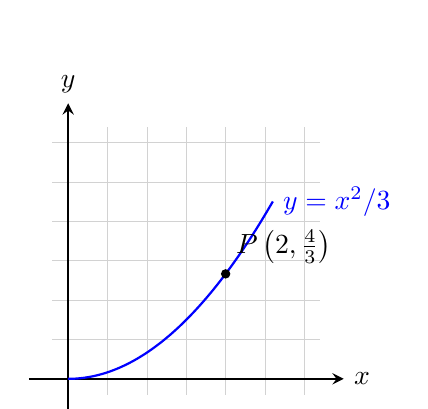
\begin{tikzpicture}[scale=1]
    \draw[gridhelp, step=0.5] (-0.2,-0.2) grid (3.2,3.2);
    \draw[arrow] (-0.5,0) -- (3.5,0) node[right] {$x$};
    \draw[arrow] (0,-0.5) -- (0,3.5) node[above] {$y$};
    \draw[domain=0:2.6, smooth, variable=\x, blue, thick]
      plot ({\x}, {\x*\x/3}) node[right] {$y = x^2/3$};
    \node[point] (P) at (2,4/3) {};
    \node[above right] at (P) {$P\left(2,\tfrac{4}{3}\right)$};
  \end{tikzpicture}
  \caption{간단한 함수 그래프 예시}
  \label{fig:parabola}
\end{figure}

\section{표}

\begin{table}[H]
  \centering
  \begin{tabular}{lcc}
    \toprule
    항목 & 측정값 & 오차 \\
    \midrule
    A & 12.30 & 0.05 \\
    B & 9.87  & 0.02 \\
    C & 15.40 & 0.10 \\
    \bottomrule
  \end{tabular}
  \caption{예제 표 (\texttt{booktabs} 사용)}
\end{table}

\end{document}
